% Created 2017-08-07 Mon 23:26
\documentclass[11pt]{article}
\usepackage[utf8]{inputenc}
\usepackage[T1]{fontenc}
\usepackage{fixltx2e}
\usepackage{graphicx}
\usepackage{longtable}
\usepackage{float}
\usepackage{wrapfig}
\usepackage{rotating}
\usepackage[normalem]{ulem}
\usepackage{amsmath}
\usepackage{textcomp}
\usepackage{marvosym}
\usepackage{wasysym}
\usepackage{amssymb}
\usepackage{hyperref}
\tolerance=1000
\newcommand{\T}{\top}
\newcommand{\E}{\ensuremath{\mbox{E}}}
\newcommand{\R}{\ensuremath{\mathbb{R}}}
\newcommand{\one}{\ensuremath{\mathbbm{1}}}
\newcommand{\Eq}[1]{(\ref{eq:#1})}
\renewcommand{\vec}[1]{\boldsymbol{#1}}
\usepackage[backend=biber,style=authoryear,natbib=true]{biblatex}
\addbibresource{prospectus.bib}
\addbibresource{main.bib}
\newcommand{\Fig}[1]{Figure \ref{fig:#1}} \newcommand{\Tab}[1]{Table \ref{tab:#1}}
\usepackage{bbm}
\usepackage{stringstrings} \renewcommand{\cite}[1]{\caselower[q]{#1}\citet{\thestring}}
\author{Elliott Collins and Ethan Ligon}
\date{February 23, 2016}
\title{Asset Transfers and Household Neediness in South Sudan}
\hypersetup{
  pdfkeywords={},
  pdfsubject={},
  pdfcreator={Emacs 24.5.1 (Org mode 8.2.10)}}
\begin{document}

\maketitle
\begin{abstract}
What happens when you give an `ultra-poor' household a productive
asset, with training in how to use it?  The answer depends on the
ways in which markets are incomplete.  Previous studies have found
that in some settings this sort of program can have a significant
impact on occupational choice and average income.  Here we document
the effects of such a program in South Sudan, but with a focus on
the \emph{welfare} of the household, using a measure related to the
household's marginal utility of expenditures, or what \cite{ligon16a}
calls the households' neediness.

This construction allows us not only to see if the the program has a
significant effect on household welfare, but also allows us to draw
inferences regarding which households would benefit most from a
hypothetical cash transfer.  We use the fact that neediness is
related not only to consumption expenditures, but also to key
variables such as the marginal product of labor, investment, and
participation in both market- and self-employment.

We report the results of an experiment which randomly assigns
participation in such a program, and find large and significant
effects on expenditures and a 0.2 standard deviation reduction in
average neediness.  These improvements in welfare are mirrored by
increases in the number and value of assets held; increases in
self-employment and skilled market employment, these last
compensated for by a marked decrease in casual agricultural labor
(and, less confidently, by an increase in leisure).
\end{abstract}

\section*{Introduction}
\label{sec-1}
We consider a program in South Sudan which provides training and
productive assets to women in very poor households, which is
intended to encouraging these women to create a productive
enterprise.  We have reasonably good data on the cost of this
program to the NGO that has implemented it.  Our question: how can
we best measure the benefit?

We consider this question from the point of view of a given
household.  We think of this household as solving a dynamic program
by simultaneously making decisions regarding consumption,
investment, occupation, and production.  All of these decisions are
tied together by a quantity \cite{ligon16a} calls `neediness', which
is simultaneously equal to the marginal benefit of additional
consumption expenditures, time, investment, and inputs to
production.  We use data on disaggregate household expenditures and
methods devised by \cite{ligon16a} to measure changes in the
logarithm of household neediness.

We find that the program results in a statistically significant 0.2
standard deviation reduction in the average log neediness of the
treatment group relative to a control group, mirroring a 6.5 SSP
(South Sudanese Pounds; about \$1.62 USD) increase in the subset 
of daily household expenditures we observe.  Other changes
can be interpreted using our model, even when they're not
necessarily predicted by that model.  Those changes include some
increase in both the number and value of productive assets held by
the treated households, and a substitution away from casual
agricultural labor into more skilled forms of market labor,
self-employment, and perhaps leisure.  Importantly, our estimates of
these other changes can use estimated household neediness as an
additional household covariate, which gives us a simple way to
distinguish between `wealth' and `substitution' effects due to the
treatment.

\section*{Background on `TUP' and Related Interventions}
\label{sec-2}

Impoverished women in underdeveloped regions tend to be involved in
low-return occupations, and frequently face both financial and human
capital constraints \citep{duflo2007}. A set of programs designed specifically
to reduce poverty typically aim to alleviate these constraints simultaneously is the ``ultra-poor graduation''
framework, in which very poor individuals are offered both physical
capital and some form of training or education to promote a particular
kind of microenterprise activity. Broad outcomes for similar programs are described in
\citep{banerjee2015}.  \cite{bandiera2017} describes a
large ultra-poor graduation initiative implemented in Bangladesh known
as the ``Transfers to the Ultra-Poor'' (TUP) program. The program was
implemented in 2007 by BRAC (cf., \url{www.brac.org}). Exploiting
the randomized pattern of expansion, the study found persistent
impacts on productivity, earnings, and participation in
microenterprise.

Subsequently, BRAC decided to pilot a TUP program near the town of
Yei in South Sudan.  This paper uses randomized enrollment to evaluate the
effects of this pilot program over the course of a year.\footnote{A more complete description
  of the experiment and the program may be found in
  \cite{Chowdhury-etal15}} In late 2013, the program gave 249 women
start-up capital at a marginal cost of around \$240. Participants
received some form of livestock, agricultural material, or retail
inventory. They then participated in training specific to the
assets provided and were given periodic food support valued at \$110.

The TUP program in South Sudan is a pilot program.  As with other
programs of its kind, it consists of four phases: targeting and
selection, training and enterprise selection, asset transfers, and
monitoring.  Each of these phases is modeled after the process in the
original program in Bangladesh, but has been modified in notable ways
based on local conditions.

\subsection*{Targeting and Selection}
\label{sec-2-1}

The TUP program in Bangladesh targeted women based primarily on a
participatory appraisal activity in which community members used
subjective means to assign households to different wealth quantiles.
By contrast, the TUP program in South Sudan relies primarily on a set
of inclusion and exclusion criteria based on wealth correlates taken
from a community-wide survey, de-emphasizing relative measures of
poverty in favor of absolute criteria.               

Targeting guidelines include characteristics correlated with poverty
as both exclusion and inclusion criteria. Surveyed households are
excluded on the basis of having a salaried worker in the household or
participation in another NGO program. Participation is also limited to
women with access to cultivable land, since this is necessary for some
of the TUP enterprises.  Of these women, BRAC identified as eligible
650 who fit at least three of the following criteria: (i) the household
head works as a day laborer; (ii) the household has two or more
children; (iii) at least one child is working; (iv) the household has fewer
than three rooms; and (v) the household includes an adult female
who has not completed secondary school.

Eligibility was established in a census conducted in April of 2013. A baseline
survey was then conducted among eligible women in June and July, which provided
stratification data for the random selection of 250 women into the TUP program,
with 375 remaining as controls.

\subsection*{Training and Enterprise Selection}
\label{sec-2-2}

Of the eligible households, 250 were randomly selected to participate
in the TUP program. After a general orientation to familiarize them
with the program overall, each client was asked their preference over
a menu of possible business types, which included selling dry fish at
market, raising goats, raising ducks, and growing maize. BRAC set the
number of participants in each group beforehand, ensuring that many
but not all participants received their preferred asset type.  Next,
clients were enrolled in business skill training. Some of this
training is program-wide, such as basic and financial literacy,
though most of it is specific to the type of asset provided.  Training
occurred over four days at BRAC's own office or demonstration farm.

\subsection*{Asset Transfer and Monitoring}
\label{sec-2-3}

The standard program then provided clients with productive assets,
with an effort to keep the market value of transferred goods constant
across enterprises. In late 2013, each client in each enterprise group
received assets valued at roughly \$240.

After transfers were made, BRAC also provided weekly food transfers
(bags of maize or maize flour) during group meetings. This was
intended to ease clients' household budgets, compensate them for
their time at trainings, and encourage them not to sell productive
assets before their businesses got off the ground. These food
transfers continued until about a month before the follow-up survey, and were
valued at roughly \$110 per client, raising the value 
of physical transfers to \$350.  BRAC estimates a marginal cost for
an additional client equal to the value of transfers plus 10--20\% of
this in delivery and administrative costs.  Initial intensive
training sessions later gave way to monitoring and mentorship from
local staff, as well as small support groups consisting of 8--12
clients, such as those found in BRAC's microfinance programs. These group meetings
were ongoing when the final round of data was collected.

\section*{Data and Selection}
\label{sec-3}

Our data comes from three principal sources.  First is a census of adult women
proximate to BRAC's regional office in Yei, which was conducted in April of 2013.
From this census a subset of 745 `eligible' women was identified, who were then
selected to be surveyed in a second `baseline' survey conducted in June and July of
the same year. This baseline identified 649 of the eligible women, who were
stratified by baseline asset holdings, participation in 
small trade and agriculture, and number of income earners, with 250 households
being randomly selected. A third follow-up survey was subsequently conducted in
July of 2014.

The first round of data collection consisted of a census of women in
households within a six kilometer radius of the regional BRAC
office.  These women typically live on small plots of land with
several small, mud, one-room buildings with thatched roofs.  Eighty
percent of surveyed women are between the ages of 20 and 40, with
between one and three children.

The census survey was designed to establish program eligibility.
BRAC's approach of selecting on a range of `correlates' of poverty
is designed to be less costly than the more intensive
community-based ranking exercise used in the Bangaladesh program,
raising the question of targeting effectiveness.  Do the eligibility
requirements sucessfully separate out an especially poor group of
women, and does it avoid excluding women who should be eligible? Of
the 1,279 surveyed households, 58\% met all of the eligibility
requirements.  A straightforward comparison of the sample averages
between the selected and non-selected groups indicates that selected
households are 17\% less likely to have paid work, have fewer
durable assets and less livestock, and are more likely to be eating
sorghum, which is typically regarded as low-quality food.  Most
selected women work either as a housewife or in small-scale
agriculture. Eighty percent lived in households with some
agricultural output, 35\% had some poultry or livestock, and roughly
36\% were involved in small trade or retail.  Average reported daily
consumption expenditures amounted to roughly \$1.50 USD per person.

Summary statistics for surveyed eligible women are presented in
\Tab{summary_statistics}, by treatment group.  The table provides
means of various outcome variables at baseline.  The column ``\(N\)''
indicates the number of non-zero values across the entire sample;
the column ``Diff.'' gives the difference in means across these two
groups, while \(p\) is related to a test of the hypotheses that
``Diff.'' is equal to zero.

\begin{longtable}{lrrrrr}
\caption{\label{tab:summary_statistics}Means of some analysis variables at baseline.  Asterisks in the column labeled ``Diff.'' are an indication of a significant difference between the means reported in the ``CTL'' and ``TUP'' columns.}
\\
 & $N$ & CTL & TUP & Diff. & $p$\\
\hline
\endhead
\hline\multicolumn{6}{r}{Continued on next page} \\
\endfoot
\endlastfoot
Consumption &  &  &  &  & \\
\hline
Meat & 378 & 4.19 & 3.64 & -0.552 & 0.11\\
Fuel & 456 & 0.74 & 0.72 & -0.017 & 0.83\\
Clothesfootwear & 595 & 0.68 & 0.64 & -0.036 & 0.62\\
Soap & 536 & 0.47 & 0.47 & 0.0 & 0.99\\
Fish & 474 & 2.46 & 2.35 & -0.107 & 0.61\\
Charities & 134 & 0.03 & 0.02 & -0.006 & 0.46\\
Cereals & 605 & 9.27 & 8.24 & -1.03 & 0.19\\
Transport & 193 & 0.18 & 0.14 & -0.033 & 0.30\\
Cosmetics & 468 & 0.64 & 0.71 & 0.065 & 0.49\\
Sugar & 604 & 1.66 & 1.64 & -0.02 & 0.91\\
Egg & 276 & 1.11 & 1.00 & -0.103 & 0.47\\
Oil & 613 & 1.32 & 1.23 & -0.087 & 0.59\\
Ceremonies & 152 & 0.14 & 0.14 & -0.002 & 0.97\\
Beans & 192 & 0.77 & 0.93 & 0.163 & 0.32\\
Fruit & 272 & 0.69 & 0.60 & -0.09 & 0.29\\
Textiles & 376 & 0.17 & 0.15 & -0.021 & 0.35\\
Utensils & 442 & 0.25 & 0.24 & -0.011 & 0.70\\
Dowry & 126 & 1.28 & 1.23 & -0.049 & 0.89\\
Furniture & 368 & 0.21 & 0.18 & -0.028 & 0.39\\
Salt & 617 & 0.45 & 0.42 & -0.028 & 0.39\\
Vegetables & 471 & 1.49 & 1.38 & -0.11 & 0.41\\
\hline
Asset Values &  &  &  &  & \\
\hline
Smallanimals & 123 & 198.90 & 150.53 & -48.368 & 0.36\\
Tv & 42 & 36.28 & 45.94 & 9.659 & 0.54\\
Bicycle & 171 & 105.58 & 96.52 & -9.06 & 0.65\\
Shop & 44 & 85.46 & 79.41 & -6.043 & 0.89\\
Radio & 260 & 53.39 & 52.48 & -0.908 & 0.94\\
Motorcycle & 93 & 450.07 & 534.69 & 84.621 & 0.48\\
Mosquito Nets\ldots{} & 423 & 19.24 & 19.83 & 0.592 & 0.77\\
\ldots{}Some treated & 181 & 8.18 & 9.04 & 0.854 & 0.56\\
Poultry & 161 & 39.68 & 39.04 & -0.642 & 0.94\\
Sewing & 28 & 8.56 & 4.96 & -3.597 & 0.42\\
Shed & 9 & 1.85 & 0.02 & -1.832** & 0.03\\
Bed & 521 & 251.30 & 249.26 & -2.039 & 0.94\\
Chairtables & 531 & 207.89 & 177.42 & -30.476 & 0.31\\
Carts & 17 & 2.31 & 3.48 & 1.173 & 0.45\\
Fan & 16 & 3.56 & 1.84 & -1.712 & 0.28\\
Homestead & 274 & 4432.11 & 4738.73 & 306.621 & 0.77\\
Cows & 35 & 222.79 & 112.70 & -110.085 & 0.19\\
Mobile & 414 & 96.25 & 110.16 & 13.912 & 0.14\\
\hline
Other Variables &  &  &  &  & \\
\hline
Daily Food & 643 & 25.11 & 22.97 & -2.136 & 0.15\\
Daily Exp & 646 & 29.82 & 27.74 & -2.079 & 0.22\\
No. Houses & 543 & 2.87 & 2.86 & -0.006 & 0.97\\
In Business & 265 & 0.40 & 0.44 & 0.033 & 0.42\\
Cereals & 605 & 9.27 & 8.24 & -1.03 & 0.19\\
Asset Prod. & 475 & 854.03 & 624.88 & -229.151 & 0.18\\
\# Child & 594 & 3.30 & 3.38 & 0.085 & 0.61\\
Land Access (fedan) & 542 & 2.50 & 2.05 & -0.443* & 0.07\\
Asset Tot. & 603 & 1787.27 & 1712.26 & -75.011 & 0.73\\
Cash Savings & 431 & 216.07 & 265.42 & 49.352 & 0.42\\
HH size & 648 & 7.32 & 7.06 & -0.267 & 0.18\\
Cosmetics & 468 & 0.64 & 0.71 & 0.065 & 0.49\\
 &  &  &  &  & \\
\end{longtable}


Though the kind of information presented in \Tab{summary_statistics} is
more useful for thinking about magnitudes than it is for `balance'
between the two randomly assigned groups, it's nevertheless true
that mean values for these groups are generally similar.  Only one
of the differences we compute is significant by the standard of a
sequence of \(t\)-tests and 95\% level of confidence, and this
difference is instructive.  It comes in the calculation of the
average value of sheds, where the control group happens to have a
total of 8 sheds, while treatment group has only four; further,
though all of the households in the control group happen to report a
that their sheds have a positive value, only one of the four
shed-owning households in the treatment group does so.  The
probability of some kind of imbalance along these lines happening
for \emph{some} variable is quite high, and of course this is no kind of
evidence against the quality of the random number generator used to
manage the assignment.  Nevertheless, the initial difference should
be kept in mind, if only because (as we'll see in the results below)
``Sheds'' are one of the outcomes which seem to be affected by the TUP
program.

\cite{chowdhury-morel15} employ a principal component index developed by the
Consultative Group to Assist the Poor (CGAP) to evaluate the effectiveness of
targeting in this experiment. They find that that roughly half of the selected
individuals are in the bottom quartile, and nearly all are poorer than average for
their community. Exclusion criteria based on NGO participation and lack of land
ownership exclude a significant number of relatively poor women, suggesting that
this targeting method has sacrificed some targeting effectiveness for the sake of
program structure.

After the original census, two surveys (a ``baseline'' and
``follow-up'') were conducted in the summers of 2013 and 2014,
respectively.  These surveys contained modules on enterprise and
income-generating activity, household composition, food security,
and consumption of a range of food and non-food goods.

Among the 745 households identified as eligible in the census,
enumerators were able to locate and interview 649 in the baseline
survey in July 2013. It was using this baseline that households were stratified by
potentially important characteristics and randomly selected for enrollment. Asset
transfers and training began in December of 2013. In total, 554 of these were
located and interviewed in the follow-up survey in July 2014. 

Since BRAC had kept in much closer contact with the TUP participants in the
intevening months, attrition is a source of concern.

\section*{A Modest Model}
\label{sec-4}

\cite{bandiera-etal12} offer a simple static model of the behavior of
an individual.  The model itself is a version of an agricultural
household model, of the sort discussed in \cite{Singh-etal86}, but
with a focus on occupational choice, which Bandiera et al. identify as a 
critical feature in their study in Bangladesh.

Here we adopt the model of \cite{bandiera-etal12} more or less
wholesale, but extend it to allow for both time and uncertainty.  The
spirit of this extension is very similar to the ``exogenously
incomplete'' model devised by \cite{Karaivanov-Townsend14}.  However,
we interpret it as a model of \emph{household}, rather than
individual behavior, since most of the data we have to test this
model is observed at the household level.  This turns it into a
dynamic model involving both asset accumulation and occupational
choice, and we show how this extension allows us to nicely tie
together the production, consumption, and investment decisions made
by the household.

Our notation is adapted from \cite{bandiera-etal12}, with modest
changes to generalize and allow for time and uncertainty.  Households
are indexed by $j\in\mathcal{J}=\{1,2,\dots,J\}$.  In each
period the economy is in a state $s\in\mathcal{S}=\{1,\dots,S\}$;
these states evolve according to finite-state Markov process with the
probability of transitioning from state $s$ to state $r$ given by
$\pi_{sr}$.  Time is discrete, and in each period $t$ the household
derives utility from consumption of an \(n\)-vector of consumption goods
$C$ and from leisure $R$.  Utility within a period can also depend on
household characteristics $\theta$.  \cite{bandiera-etal12} interpret
this $\theta$ as skills, but we'd interpret it more broadly to include,
e.g., household size and composition.  Then momentary utility is given
by $U(C,R,\theta)$, with this utility function increasing, concave,
and continuously differentiable.  The household makes plans over an
infinite horizon, with utility in the next period discounted by a
factor $\beta\in(0,1)$.

In each period the household allocates its time between leisure $R$,
employment (by others) $L$, and self-employment $S$. All must be
non-negative.  We assume that no labor is hired in by the household
(modifying the model to allow this would be straight-forward, but not
empirically useful in our setting, as none of the households in our
sample is observed to hire in labor).  Earnings from employment
depends on an individual and state-specific function
$W^j_{s}(L,\theta)$.  Income from self-employment involves a
production process which depends not only on time allocated to this
occupation, but also on the productive assets and a
household-specific shock; household \(j\)'s characteristics evolve
according to a household-specific Markov process, so that
$\theta_{t+1}=H^j_{s}(\theta_{t})$ if the state at $t+1$ is $s$.

Asset accumulation depends on initial assets $K$, the state-specific
idiosyncratic price for new assets $q^j_s$, and stochastic, household-specific
returns to holding those assets $Q^j_{s}(K)$ (e.g., think of livestock
fertility and mortality).  Borrowing is limited, but these limits may depend on the
state and vary across households, so that $K_{t+1}\leq B^j_{s}(K_t)$
if the $t+1$ state is $s$.  The
returns function $Q^j_{s}$ is assumed to be weakly concave; both it and
the borrowing limit functions $B^j_{s}$ are also assumed to be increasing
and continuously differentiable.

In any state $s$, given assets $K$, characteristics $\theta$, and time
spent in self-employment $S$, household \(j\) produces
$F_{js}(K,S,\theta)$ units of the numéraire good, where we assume the
$F_{js}$ are increasing, weakly concave, and continuously
differentiable.  The cost of purchasing the consumption bundle $C$ is
taken to be $P^j_s(C)$ for household \(j\) in state $s$.  In each
period the cost of consumption plus net investment must not exceed
income from employment and own production, so that household \(j\) faces
the budget constraint
\begin{equation} 
\label{eq:bc}
   P^j_s(C) + q^j_s(K'-K) \leq F^j_{s}(K,S,\theta) + W^j_{s}(L,\theta),
\end{equation}
where $K'$ is a vector of the total assets invested for the next
period.

Putting this altogether, we regard household \(j\) as solving the
dynamic program
\begin{equation}
\label{eq:bellman}
  V^j_{s}(K,\theta)=\max_{C,S,L,K'} U(C,1-L-S,\theta) +
  \beta\sum_{r\in\mathcal{S}}\pi_{sr}V^j_{r}\left(Q^j_{r}(K'),H^j_{r}(\theta)\right)
\end{equation}
subject to the budget constraint \Eq{bc} (with which we associate the
Karush-Kuhn-Tucker multipliers \(\lambda^j_s\)); to non-negativity
constraints on consumption goods $i=1,\dots,n$, (with associated
multipliers $\nu_i^j$); non-negativity constraints for time
allocation $S\geq 0$ and $L\geq 0$ (with multipliers $\eta^j_S$ and
$\eta^j_L$, respectively); and subject finally to the borrowing
constraint $K'\leq B^j_{s}(K)$ (with multipliers \(\mu^j_s\)).

Using lower case letters to indicate partial derivatives, the first order conditions then can be written
\begin{equation}
\label{eq:foc}
\begin{aligned}
  C_i &: u_i(C,R,\theta) - \nu^j_i &=& p^j_{si}\lambda^j_s \qquad\text{for all $i=1,\dots,n$}\\
  L   &: u_R(C,R,\theta) - \eta^j_L &=& w^j_s\lambda^j_s\\ 
  S   &: u_R(C,R,\theta) - \eta^j_S &=& f^j_{S}\lambda^j_s \\
  K'  &: \beta\sum_r\pi_{sr}v^j_{r}q^j_{r} + \mu^j_s &=& q^j_{s}\lambda^j_s.\\
\end{aligned}
\end{equation}
Here $u_i$ denotes the marginal utility of consumption good $i$, and $u_R$
is the marginal utility of leisure.  Similarly $f^j_{s}$ is the marginal
product of $S$ in production for household \(j\), while $v^j_{r}=\frac{\partial
   V^j_{r}}{\partial K}(Q^j_{r}(K'),H^j_{r}(\theta))$ is household \(j\)'s
marginal valuation of an additional unit of realized capital in state
$r$, and $q^j_{r}$ is \(j\)'s marginal return to investment in state
$r$.  In addition to these optimality conditions we have the envelope
condition with respect to $K$,
\begin{equation}
\label{eq:env}
  v^j_{s}(K,\theta) - \mu^j_sb^j_s(K) = \lambda^j_s\left(q^j_s + f_{sK}(K,S,\theta)\right).
\end{equation}

Now, the key variable which ties together all of these is the
multiplier on the budget constraint, which measures the marginal
benefit of having additional resources.  Since this marginal value
depends in turn on not only the state $s$ but also the current values
of $(K,\theta)$, we use \Eq{foc} and \Eq{env} to implicitly write it as a
function $\lambda^j_s(K,\theta)$.  We have
\begin{equation}
\label{eq:returns}
   \lambda^j_s(K,\theta) = \frac{u_i - \nu^j_i}{p^j_{si}} = \frac{u_R - \eta^j_L}{w^j_s} =
   \frac{u_R-\eta^j_S}{f^j_{sS}}=\frac{\beta\sum_r\pi_{sr}v^j_{r}q^j_{r} +
     \mu^j_sb^j_s}{q^j_s} = \frac{v^j_{s}-\mu^j_sb^j_s}{q^j_s + f^j_{sK}}.
\end{equation}
In words, the household is allocating its resources to equate returns
measured in terms of \emph{utility} across different margins; none of
these are returns in physical quantities that we can directly measure.
``Utility return'' would be an accurate way of describing these
quantities: Taking each equality in \Eq{returns} one at a
time, $\lambda^j_s$ is equal to household \(j\)'s utility return of
consuming an additional unit of good $i$ (this holds for every
$i=1,\dots,n$, of course); is equal to the utility return to taking an
hour off from employment; is equal to the utility return to taking an
hour off from self-employment; and is equal to the utility return to
an additional unit of investment, which finally is equal to the
utility value of having additional assets in the current state $s$.

But while ``utility return to an additional unit of investment'' may
be accurate, we think the English language already has a suitable
word: the variables $\lambda^j_s$ measure the \emph{neediness} of
household \(j\).  When $\lambda^j$ is high relative to those of other
households, so is $(u^j_i-\nu^j_i)/p^j_i$, and household \(j\) stands in greater
need of food; similarly when $\lambda^j_s>\E\lambda^j$ the household
is particularly in need of labor; of investment; of consumption; of
leisure. 

The neediness variables $\lambda^j_s$ have other interpretations as
well.  If we were to consider the static consumer's problem being
solved by household $j$ at each  date state, then $\lambda^j_s$ is
equal to the partial derivative of the household's indirect utility
function with respect to total consumption expenditures in state $s$.

Notice that the different expressions for neediness in \Eq{returns}
involve three different kinds of objects.  First, there are some
prices which may be directly observable in the data (e.g., prices of
consumption goods; individuals' wages; purchase prices of assets such
as livestock).  Second, there are shadow prices that will \emph{not}
be directly observable; these include the key $\lambda^j_s$ as well as
multipliers on the non-negativity constraints and the multiplier on
the borrowing constraint.  Third, there are unknown functions,
including the marginal utility functions $(u_i,u_R)$ and the marginal
productivities of assets and labor in the self-employment technology
$(f^j_{sS},f^j_{sK})$.

\subsection*{Modeling our experiment}
\label{sec-4-1}

We want to think now about how our experiment can be thought of in
terms of the model of the households we've developed---only by putting
the experiment ``into'' the model can we think coherently about how a
household might react to the experimental treatments we introduce.  Or
as \cite{Rubin74} might put it, we think of putting the experiment
into the model as the construction of a logical argument establishing
circumstances under which only some particular variables should be
expected to have a causal effect on particular dependent variables.

Accordingly, consider partitioning the space
$\mathcal{S}=\mathcal{C}\cup\mathcal{E}$.  Then for any state
$s\in\mathcal{E}$ we begin our experiment (we can always specify
\(\mathcal{S}\) and choose the transition probabilities $\pi_{sr}$ to
ensure that we only start the experiment once).  Further, let $T_0(s)$
and $T_1(s)$ be subsets of the index set of households, so that for
$\hat s\in\mathcal{E}$ if $j\in T_0(\hat s)$ then household \(j\) is
assigned to a `control group' in our experiment, while if $j\in
T_1(\hat s)$ then household \(j\) is assigned to a `treatment group'
which receives assets, training, and so on.  Assignment is random if,
for any pair of households $(j_0,j_1)\in T_0\cup T_1$ each had an
equal probability of being assigned to $T_1$.

In partitioning $\mathcal{S}$ into states where the experiment is
conducted and states where it is not, we think of $\mathcal{C}$ as the
set of `counterfactual' states.  Thus, for an `experiment' state $\hat
s\in\mathcal{E}$ there exists another `counterfactual' state $\tilde s\in\mathcal{C}$
such that for any household $j\in T_1(\hat s)$, the `treatment'
consists of an $\hat K$, a $\hat\theta$, and a $\hat C$ such that
\begin{equation}
\label{eq:treatment_counterfactual}
   Q^j_{\hat s}(K') =    Q^j_{\tilde s}(K') + \hat K; \quad
   H^j_{\hat s}(\theta) = H^j_{\tilde s}(\theta) + \hat\theta;\quad
   \text{and $P^j_{\hat s}(C) = P^j_{\tilde s}(C-\hat C)$}
\end{equation}
for all $K'$, $\theta$, and $C$. Note that we are \emph{not} assuming
that consumption or investment will be unchanged by the treatment; it
would be surprising if they were not.  The content of the assumption
is that the technology producing returns to investment or the cost of
a consumption bundle only be affected by the experiment in an additive
way.  

Further, we assume that for any household in the \emph{control} group
outcomes are the same in both the experimental state $\hat
s\in\mathcal{E}$ and the counterfactual state $\tilde
s\in\mathcal{C}$, or, for any $j\in T_0(\hat s)$ that we have
\begin{equation}
\label{eq:control_counterfactual}
   Q^j_{\hat s}(K') =    Q^j_{\tilde s}(K'); \qquad
   H^j_{\hat s}(\theta) = H^j_{\tilde s}(\theta);\qquad
   \text{and $P^j_{\hat s}(C) = P^j_{\tilde s}(C)$,}
\end{equation}
also for all $K'$, $\theta$, and $C$.  Together, these two conditions
just assert that our experiment only affects the treated, and give the
effect of the treatment on treated households.  Left unstated is a
third assumption, that the treatment's effects on treated households
are channeled solely through the transfers of $(\hat K,\hat\theta,\hat
C)$.



This notation may seem unnecessary, if our goal is simply to discuss
what it means to have experimental treatments and random assignments.
But now we ask---within the context of the model---what effects we'd
expect from the experimental treatment.  There turns out to be a very
simple way to measure these.  Equation \Eq{returns} implies that
changes in any aspect of the household's economic behavior
(consumption, labor supply, production, credit constraints) will be
reflected in the neediness $\lambda^j_s$, so one way of thinking about
what we want to measure experimentally is the ratio $\lambda^j_{\hat
s}/\lambda^j_{\tilde s}$ for $j\in T_1(\hat s)$.  This ratio would
tell us the proportional difference in utility returns for a treated
household due to the experiment.

Viewed through this lens, the expected ``average treatment effect''
on (the log of) neediness can be written as
\[
   \mbox{ATE}=\E\left(\frac{1}{\#T_1(\hat s)}\sum_{j\in T_1(\hat s)}\log\lambda^j_{\hat s}\right) - \E\left(\frac{1}{\#T_1(\hat s)}\sum_{j\in T_1(\hat s)}\log\lambda^j_{\tilde s} \right).
\]
The problem, of course, is that we can't observe the \(\lambda^j\)s in
the counterfactual state $\tilde s$.  But using the assumption
\Eq{control_counterfactual} and the assumption of random assignment,
it follows that 
\[
   \E\left(\frac{1}{\#T_1(\hat s)}\sum_{j\in T_1(\hat
       s)}\log\lambda^j_{\tilde s} \right)=\E\left(\frac{1}{\#T_0(\hat
       s)}\sum_{j\in T_0(\hat s)}\log\lambda^j_{\hat s} \right), 
\]
so that we have the average treatment effect on the logarithm of
neediness given by 
\begin{equation}
\label{eq:ate}
    \mbox{ATE}=\E\left(\frac{1}{\#T_1(\hat s)}\sum_{j\in T_1(\hat s)}\log\lambda^j_{\hat s}\right) - \E\left(\frac{1}{\#T_0(\hat s)}\sum_{j\in T_0(\hat s)}\log\lambda^j_{\hat s} \right).
\end{equation}
This now only involves needing to observe outcomes in realized states.


\section*{Empirical Strategy}
\label{sec-5}

Notice that the utility returns in \Eq{returns} involve three
different kinds of objects.  First, there are some prices which may be
directly observable in the data (e.g., prices of consumption goods;
individuals' wages; purchase prices of assets such as livestock).
Second, there are shadow prices that will \emph{not} be directly
observable; these include the key $\lambda^j_s$ as well as multipliers
on the non-negativity constraints and the multiplier on the borrowing
constraint.  Third, there are unknown functions, including the
marginal utility functions $(u_i,u_R)$ and the marginal productivities
of assets and labor in the self-employment technology
$(f^j_{sS},f^j_{sK})$.

These last unknown functions depend on variables which we may be able
to observe.  Consider in particular a good $i$ of which household $j$
consumes a positive quantity.  This gives us the equality
$u_{i}(C^j_s,R^j_s,\theta^j_s)/p^j_{si}(C^j_s)=\lambda^j_s$.  This
equation holds for all states and for every good $i=1,\dots,n$ with
positive consumption, so it must hold in any realized state.  To
celebrate this fact we simplify notation, letting $t$ indicate the
state that occurs at that date, so that we have
$u_{i}(C^j_t,R^j_t,\theta^j_t)/p^j_{ti}(C^j_t)=\lambda^j_t$ to
indicate this relationship at date $t$ and state $s_t$.  With this
simplified notation we also introduce some additional assumptions:
first, that utility from leisure is additively separable from utility
from consumption, or that $u_{iR}=0$.  Second, we partition the index
set of households into sets of households that reside within $m$
distinct areas; i.e., we take
$\mathcal{J}=\mathcal{J}_1\cup\mathcal{J}_2\cdots\cup\mathcal{J}_m$.
Then we assume that within each of these $m$ areas households all face
the same prices for consumption goods, or that $p^j_{ti}(C^j)=p_{ti}$.

Now, with this we return to the equation defining the expected average
treatment effect  \Eq{ate}.  Using the fact that for goods consumed in
positive amounts we now have
$\lambda^j_t=u_i(C^j_t)/p_{ti}$, we substitute into \Eq{ate},
obtaining
\[
   \log u_i(C^j_t,\theta^j_t) = \log p_{ti} + \sum_g\one(j\in T_g)\overline{\log\lambda_t}^{T_g} + \epsilon^j_{ti},
\]
where $\overline{\log\lambda_t}^{T_g}$ is the average value of the
\(\log\lambda\)s for treatment group $T_g$,
$\epsilon^j_{ti}$ is a residual which, by \Eq{ate} will be equal to
$\lambda^j_t-\overline{\log\lambda_t}^{T_g}$ if household \(j\) is a member
of treatment group $g$.

\subsection*{Estimating Marginal Utilities}
\label{sec-5-1}

If we observed prices $p_{ti}$ and happened to know the values of
$\log u_i(C^j_t,\theta^j_t)$ we could go ahead and straight-forwardly
estimate the average treatment effect we're interested in.  Of course
we do not know the latter.  However, we do observe expenditures on
multiple kinds of food and other non-durable consumption.  If we
re-arrange the first equality in \Eq{returns} and use our assumption
that leisure is separable in utility then we can write the vector of
marginal utilities of consumption as \[ u(C,\theta)=p\lambda.  \]
Next, following the long line of work following
\cite{Heckman-Macurdy80} and \cite{Macurdy83}, we parameterize the log
of marginal utilities, assuming $\log u(C,\theta)=\Gamma\log C +
\zeta\theta$, where $\Gamma$ is an $n\times n$ matrix of parameters
having full rank, and where $\zeta$ is an $n\times l$ matrix.\footnote{The
development and justification of this particular preference structure
is discussed in \cite{ligon15}.}

With this parameterization, we can write \[ \Gamma\log C + \zeta\theta
= \log p + \log\lambda.  \] This is getting close to something we can
estimate, but we have data on the value, not quantity, of food
consumption.  Let $X_i=p_iC_ie^{\epsilon_i}$, where $\epsilon_i$ is
some measurement error, be the value of expenditures on consumption
good $i$.  Then rearranging, we have the system of equations
\begin{equation}
\label{eq:expenditures}
\log X  = (I + \Gamma^{-1})\log p - \Gamma^{-1}\zeta\theta + \Gamma^{-1}\log\lambda
+ \epsilon.
\end{equation}
This system is what we might call a Frischian expenditure system
\citep{browning-etal85}.  \cite{ligon16a} provides methods for
estimating this system; showing that with data on at least some
expenditures and household characteristics one can obtain not only
estimates of the parameters but also of the neediness measures
$\log\lambda$ (up to a normalization).

Differences in the mean of the inferred neediness $\log\lambda$ between
treatment and control group will be equal to the average treatment
effect that most interests us, but we can also obtain estimates of
this effect directly from \Eq{expenditures}.  Consider the following
standard ANCOVA specification of the sort championed by
\cite{Mckenzie2012}.  Key features of the standard specification
include a set of fixed effects for time and place; linear covariates
as controls; baseline values of the outcomes as additional controls;
and finally a collection of average treatment effects, which are
ordinarily the object of interest.  We adopt just such a
specification, letting $X^{jga}_{ti}$ be expenditures on good $i$ in
period $t$ for a household \(j\) in area $a$ and in treatment group $g$.
Then we can write
\begin{equation}
\label{eq:ancova}
  \log X^{jga}_{ti} = \alpha^a_{ti} + \tau^g_i +  \delta_i(\theta^j_t - \bar\theta^g_t) + \gamma_i \log X^{jga}_{t-1,i} + u^j_{ti}.
\end{equation}
Now, in the standard interpretation of this regression $\tau^1_i-\tau^0_i$
will be the average treatment effect on expenditures on good $i$, while the terms
involving the $\theta$ and the lagged outcomes improve power by
accounting for covariance between household characteristics and
expenditures (and perhaps accounting for unbalanced outcomes in the
baseline).  Because the latent variables $\alpha^a_{ti}$ capture
differences in means across areas as well as goods and periods, it is
the variation that is within an area that is being exploited here to
estimate the $\tau^g_i$.

This ANCOVA specification has an intimate relationship with the
Frischian expenditure system \Eq{expenditures} which allows us to give
a structural interpretation of the reduced-form ANCOVA.  In
particular, the good-area-time effects $\alpha^a_{ti}$ estimate the
effects of changes in prices on expenditures, the vector
$(I + \Gamma^{-1})\log p_{t}$ in \Eq{expenditures}.  The terms involving
the idiosyncratic covariate characteristics $\delta_i\theta^j_t$ match
up with the effects of characteristics on expenditure demand
$\Gamma^{-1}\zeta\theta_t$, while the average treatment effect
estimates $\tau^g_i=\beta_i(\overline{\log\lambda_t}^{T_1} +
\zeta_i\bar\theta^g_t)$, where the $\beta_i$
are equal to the row sums of the matrix $\Gamma^{-1}$. 

So, the average treatment effect in these ANCOVA regressions with log
consumption expenditures as outcomes can be interpreted as the product
of a demand elasticity and neediness.  Further, these can be
decomposed, giving us both parameters useful for understanding demand
systems and Engel curves and measures of neediness useful for
measuring welfare.  Even better, these neediness parameters are key to
understanding the connections between consumption, investment,
production, and occupational choice, and allow us to measure
the extent to which an intervention operates via its effects on wealth
versus effects it may have on production or occupational choice.

What assumptions have we had to make in order to give this
`structural' interpretation to our average treatment effects?  There
are only really four `structural' assumptions we need to make.  All
pertain to the household's utility function, and seem fairly
unobjectionable, or at least conventional in applied empirical work.
The first two are that the household's utility function is
intertemporally separable and von Neumann-Morgenstern; these allow us
to think of the household as solving a `two-stage' intertemporal
budgeting problem \citep{gorman59}. The third is that the utility function is separable
in consumption and leisure; the last that Frischian consumption
expenditure elasticities are constant.  This is much less restrictive
than what is usually assumed in parametric Engel curve estimation.

\section*{Results}
\label{sec-6}

We offer results in three parts.  First we discuss the average
treatment effect on consumption expenditures, and use estimates of
this effect across different consumption goods to estimate the average
treatment effect on neediness, as well as the distribution of
neediness in both treatment and control groups.  Second, we consider
outcomes related to both the number and value of assets held by the
household.  The estimates of household neediness previously obtained
can be used to control for the effects of treatment on wealth.  The
link between these holdings and the model is considerably looser than
in the case of consumption, but certainly both the average number and
value of assets we observe is positively affected by TUP.  The
distribution of resources \emph{across} different assets is less easy to
predict, but we see large average treatment effects on the value of
livestock owned, consistent with the focus of TUP on increasing
livestock ownership for treated households which choose this.  We
finally examine self-employment and occupation.  There are quite large
effects on participation in self-employment, broadly consistent with
what one would expect from a purely administrative analysis (BRAC gave
animals to so many treated households, of which a certain known number
already had significant livestock holdings).  Finally, we turn to a
broader and more detailed notion of occupation: here we see members of
treated households leaving housework and casual agricultural
employment.  Some of these people seem to enter non-agricultural day
labor, but it's less clear what they're doing instead.  However, one
possibility consistent with both the evidence and the model is that
people in the average treated household move out of low-skill market
employment, instead increasing labor in more skilled market
employment, and possibly increasing both household leisure and
participation in home production.

\subsection*{Consumption Expenditures and Neediness}
\label{sec-6-1}

Our principal results may be found in \Tab{goods_results}.  As
suggested above, these are `ANCOVA' estimates of the effects of being
in either of the two groups ``CTL'' (Control) and ``TUP'' (targeted
ultra-poor), the latter of which received assets, training, and food
subsidies.  Other household characteristics included as controls
are the number of people in the household as well as the number of
children.  Baseline values of expenditure were included as an
additional control, with a complete set of village/area fixed effects
(constrained to sum to zero).  Where recorded values of consumption
expenditure are equal to zero, these are regarded as missing and
dropped from the analysis.  There are two motivations for this
treatment of zeros: first, at an entirely practical level, our
dependent variable is the logarithm of expenditures, which is
undefined at zero.  But second, if a household is at a corner when it
chooses a particular consumption item, then the first order condition
in \Eq{foc} for that consumption good won't be correct (we'd be
missing a multiplier related to non-negativity).  By simply dropping
observations for goods where consumption is zero we are effectively
dropping observations where expenditures do not correctly reveal
household neediness.  In any event, treating zero consumptions as
missing results in our `panel' of goods by households being
unbalanced, so we estimate the ANCOVA equations as a single system.

We see in the first instance that the average treatment effect for TUP
participants on the value of these consumption goods are almost
uniformly positive, and significantly positive (three stars indicates
a 99\% level of confidence, two stars 95\%, and one star 90\%) for 8 of
14 different goods.  The exceptions are informative.  The estimated
sign for the difference in the value of salt consumption is negative,
but very small and insignificant, consistent with the view that the
income elasticity of salt is very small for this population.  The
other negative difference is for transportation expenditures.  We've
included transportation in this table with the idea that
transportation services enter the utility function.  But another view
is that transportation is an expense associated with employment or
production.  One of the principal findings of \cite{bandiera-etal12}
is that TUP participants in Bangladesh switched from wage employment
to self-employment, which one presumes may have reduced the demand for
transportation, and it's very possible that something similar is
happening here.

The differences in average treatment effects are also highly jointly
significant: a test of the hypothesis that these are all zero
yields a $\chi^2_{14}$ statistic of 75.43, with an associated
\(p\)-value less than $10^{-9}$.  

\begin{table}[htb]
\caption{\label{tab:goods_results}Average treatment effects for value of consumption of different goods from ANCOVA regression, along with estimated Frisch elasticities $\beta_i$ (proportional to income elasticities).  Controls include baseline values of expenditures, household size, and numbers of children.  Asterisks indicate statistical significance at 90, 95, or 99\% level of confidence.}
\centering
\begin{tabular}{llllll}
Goods & $N$ & CTL & TUP & Diff. & $\beta_i$\\
\hline
Beans & $464.000$ & $-0.034^{**}$ & $0.033^{**}$ & $0.067^{***}$ & $0.236^{***}$\\
 &  & $(0.017)$ & $(0.015)$ & $(0.022)$ & $(0.021)$\\
Bread & $311.000$ & $-0.015$ & $0.014$ & $0.029$ & $0.252^{***}$\\
 &  & $(0.024)$ & $(0.021)$ & $(0.032)$ & $(0.033)$\\
Cosmetics & $397.000$ & $-0.079^{***}$ & $0.080^{***}$ & $0.160^{***}$ & $0.514^{***}$\\
 &  & $(0.028)$ & $(0.027)$ & $(0.039)$ & $(0.032)$\\
Egg & $91.000$ & $-0.048$ & $0.050^{**}$ & $0.098^{**}$ & $0.186^{***}$\\
 &  & $(0.044)$ & $(0.020)$ & $(0.049)$ & $(0.046)$\\
Fish & $420.000$ & $-0.034^{*}$ & $0.036^{**}$ & $0.070^{***}$ & $0.224^{***}$\\
 &  & $(0.020)$ & $(0.016)$ & $(0.026)$ & $(0.026)$\\
Fruit & $114.000$ & $-0.028$ & $0.028$ & $0.056$ & $0.234^{***}$\\
 &  & $(0.046)$ & $(0.042)$ & $(0.062)$ & $(0.059)$\\
Fuel & $521.000$ & $-0.032$ & $0.030$ & $0.062$ & $0.627^{***}$\\
 &  & $(0.034)$ & $(0.029)$ & $(0.045)$ & $(0.036)$\\
Maize & $308.000$ & $-0.063^{*}$ & $0.063^{**}$ & $0.125^{***}$ & $0.233^{***}$\\
 &  & $(0.037)$ & $(0.030)$ & $(0.047)$ & $(0.051)$\\
Meat & $169.000$ & $-0.053$ & $0.055$ & $0.109^{*}$ & $0.210^{***}$\\
 &  & $(0.042)$ & $(0.040)$ & $(0.058)$ & $(0.051)$\\
Millet & $59.000$ & $-0.044$ & $0.101$ & $0.144^{*}$ & $-3.172^{***}$\\
 &  & $(0.048)$ & $(0.070)$ & $(0.085)$ & $(0.268)$\\
Oil & $514.000$ & $-0.024$ & $0.022$ & $0.045^{*}$ & $0.322^{***}$\\
 &  & $(0.021)$ & $(0.016)$ & $(0.026)$ & $(0.024)$\\
Rice & $415.000$ & $-0.016$ & $0.016$ & $0.032$ & $0.252^{***}$\\
 &  & $(0.021)$ & $(0.018)$ & $(0.027)$ & $(0.026)$\\
Salt & $535.000$ & $0.002$ & $-0.002$ & $-0.004$ & $-0.002$\\
 &  & $(0.006)$ & $(0.004)$ & $(0.007)$ & $(0.007)$\\
Soap & $543.000$ & $-0.077^{***}$ & $0.080^{***}$ & $0.157^{***}$ & $0.635^{***}$\\
 &  & $(0.028)$ & $(0.025)$ & $(0.038)$ & $(0.026)$\\
Sorghum & $211.000$ & $-0.028$ & $0.023$ & $0.051$ & $0.171^{***}$\\
 &  & $(0.031)$ & $(0.027)$ & $(0.041)$ & $(0.039)$\\
Sugar & $513.000$ & $-0.023$ & $0.020$ & $0.043$ & $0.370^{***}$\\
 &  & $(0.021)$ & $(0.016)$ & $(0.027)$ & $(0.023)$\\
Sweetpotato & $57.000$ & $0.021$ & $-0.036$ & $-0.057$ & $0.280^{***}$\\
 &  & $(0.035)$ & $(0.060)$ & $(0.069)$ & $(0.091)$\\
Transport & $116.000$ & $0.009$ & $-0.026$ & $-0.035$ & $0.704^{***}$\\
 &  & $(0.061)$ & $(0.060)$ & $(0.086)$ & $(0.068)$\\
Vegetables & $512.000$ & $-0.054^{**}$ & $0.052^{***}$ & $0.106^{***}$ & $0.362^{***}$\\
 &  & $(0.023)$ & $(0.018)$ & $(0.029)$ & $(0.026)$\\
\hline
$\overline{\log\lambda}^g$ & $554$ & $0.138^{***}$ & $-0.060^{***}$ & $-0.198^{***}$ & ---\\
\end{tabular}
\end{table}

Now recall that according to our model each treatment effect is equal
to the product of an elasticity parameter $\beta_i$ and average log
neediness for the group.  By redefining the `treatment groups' so that
there are 554 of them, each group consisting of exactly one household,
we can obtain estimates of \emph{individual} effects on the value of goods
consumed, or $\beta_i\log\lambda^j_t$.  We adopt the normalization
that $\mbox{var}(\lambda^j_t)=1$, and scale the elasticities $\beta_i$
so that their sum weighted by expenditure shares is equal to one.
Scaled in this way these Frisch elasticities would be equal to
Marshallian income elasticities provided each household had a
coefficient of relative risk aversion of one.  These Frisch
elasticities are reported in the final column of \Tab{goods_results}.
As the differences in estimated average treatment effects would
suggest, all but salt appear to be normal goods.  Because the scale is
only identified by an arbitrary normalization, we can't say based on
this evidence what goods are necessities or a luxuries.  But we can
say that fuel, transport, soap, and cosmetics (all the non-food items)
appear to be the four most income elastic goods, followed by
vegetables, sugar, cooking oil, and cereals.  And whatever the scale,
the least income elastic good seems to be salt, with an elasticity
orders of magnitude smaller than that of the most income elastic goods.

We now turn our attention to the relationship between (log) neediness
and treatment.  The final row of \Tab{goods_results} reports the mean
values of neediness for both CTL and TUP groups.  As with the
individual goods, there's a highly significant difference between
these means.  Because the standard deviation of the pooled
$\log\lambda^j_t$ is equal to one (because of our normalization), we
can interpret the difference between these means as evidence that
neediness for the treatment group fell by a highly statistically
significant 0.2 standard deviations relative to the control.

\begin{figure}[htb]
\centering
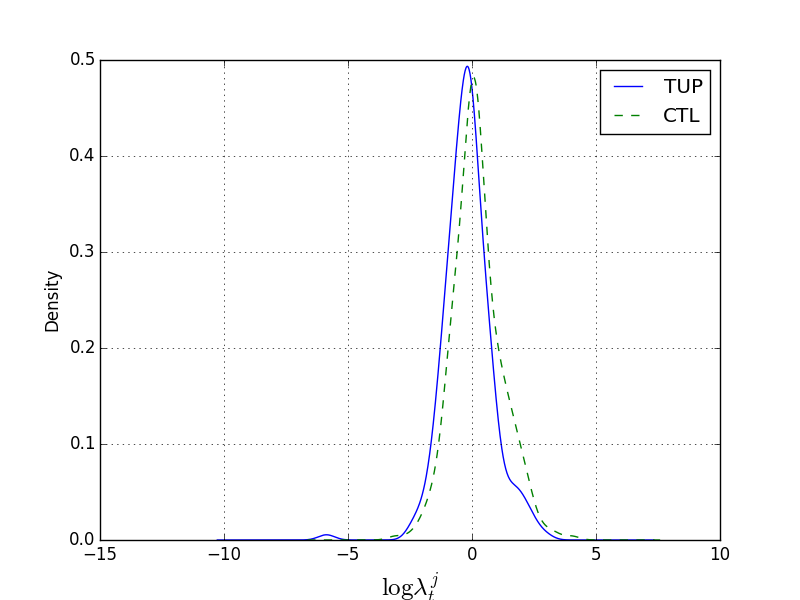
\includegraphics[width=.9\linewidth]{../analysis/figures/loglambda_distribution_by_treatment.png}
\caption{\label{fig:loglambda_distribution_by_treatment}Distribution of Neediness, by Treatment.}
\end{figure}

Of course, knowing just that the mean neediness is less in the TUP
group tells us little about how changes in welfare are distributed
across households.  Giving assets to would-be entrepreneurs might have
very disparate effects on welfare, as many standard models of
entrepreneurship predict
\citep{banerjee-newman93,paulson-etal06,karaivanov-townsend14} and as
a number of recent experiments tend to confirm \citep{demel-etal08,mckenzie-woodruff08,fafchamps-etal11}.
Perhaps some fortunate or skilled few benefit hugely while others
experience little benefit.  

To understand the distribution of benefits in our setting, consider
\Fig{loglambda_distribution_by_treatment}, which presents kernel
density estimates of the distribution of $\log\lambda^j_t$ across
households conditional on whether they are members of either the
treatment or control group.  Two things are visually evident from the
figure.  The first is that average neediness for the TUP group is
smaller than it is for the control group.  Related, the second is that
the distribution of welfare gains for the TUP group may first-order
stochastically dominate the distribution for the control group: it's
not just that mean neediness falls, it's that mean neediness appears
to fall for \emph{everyone}, save for the least needy (consistent with the
idea that the utility function $U$ is concave).  


\section*{Other Testable Predictions of the Model}
\label{sec-7}
The model presented here is written so as to be quite
general in some dimensions, and we lack the data to construct
structural estimates of the full model.  However, with only fairly
modest maintained assumptions we can estimate parts of this model,
and test others.  For example, the previous section has outlined
methods for estimating a parametric utility function and
corresponding demands for non-durable consumption, which we exploit
below.  We have also described an approach to measuring the effects
of the TUP program on average household welfare.

With what we've been able to estimate, we'd like to be able to use
the model to ask two counterfactual questions about the TUP
program.  The first: what size of cash transfer would yield the
same welfare benefits as what we observe from the experiment?
We'll call this the ``welfare-equivalent cash transfer.''  The
second: in what ways is the behavior induced by the TUP program
different from what we'd expect from the welfare-equivalent cash
transfer?


\section*{Results}
\label{sec-8}

We offer results in three parts.  First we discuss the average
treatment effect on consumption expenditures, and use estimates of
this effect across different consumption goods to estimate the average
treatment effect on neediness, as well as the distribution of
neediness in both treatment and control groups.  Second, we consider
outcomes related to both the number and value of assets held by the
household.  The estimates of household neediness previously obtained
can be used to control for the effects of treatment on wealth.  The
link between these holdings and the model is considerably looser than
in the case of consumption, but certainly both the average number and
value of assets we observe is positively affected by TUP.  The
distribution of resources \emph{across} different assets is less easy to
predict, but we see large average treatment effects on the value of
livestock owned, consistent with the focus of TUP on increasing
livestock ownership for treated households which choose this.  We
finally examine self-employment and occupation.  There are quite large
effects on participation in self-employment, broadly consistent with
what one would expect from a purely administrative analysis (BRAC gave
animals to so many treated households, of which a certain known number
already had significant livestock holdings).  Finally, we turn to a
broader and more detailed notion of occupation: here we see members of
treated households leaving housework and casual agricultural
employment.  Some of these people seem to enter non-agricultural day
labor, but it's less clear what they're doing instead.  However, one
possibility consistent with both the evidence and the model is that
people in the average treated household move out of low-skill market
employment, instead increasing labor in more skilled market
employment, and possibly increasing both household leisure and
participation in home production.

While \cite{banerjee2015} do not estimate neediness according to our procedure,
they both find comparable average treatment effects on the sum of 
consumption for the expenditure categories they measure. The consistency of average
treatment effects across the distribution also mirrors the distributional results in
\cite{banerjee2015}. \cite{bandiera2017} find increases in consumption among
the ultra-poor, but do not report short-term estimates like the ones we present here.

\subsection*{Assets}
\label{sec-8-1}

We have seen that the TUP treatment has a positive and significant
effect on consumption expenditures and leads to a significant and
sizable reduction in neediness.  From \Eq{foc}, we might expect this
reduction in neediness to also show up in investment and assets.  Of
course, since the TUP program revolves around actually giving assets
to treated households, it may appear obvious that assets should
increase.  But in fact this is not at all a foregone conclusion.  From
\Eq{foc} we have an indication that a decrease in neediness (such as
the one we measured above) may decrease the marginal value of assets
(consistent with an increase in the holdings of those assets).  But
the assets may be valued simply because they can be sold to finance
increased consumption or leisure---a pure wealth effect, which would
be reflected in a reduction in neediness $\lambda^j_s$.  This use
certainly improves welfare, and may help extend the benefits of the
TUP program to future periods, but this is a role that would be played
equally well by a (simpler) financial transfer.  For the asset
transfers to play an important role in \emph{production}, we should look
for the effects they may have on the production function, where a
transfer of particular assets may either directly enter the production
function, or may help to relax a borrowing constraint (perhaps by
serving as a security), allowing the household to finance the purchase
of other inputs to production should it wish.

Here we explore the effect of the TUP program on physical assets by
estimating the average treatment effect on both the number
(\Tab{asset_count_results}) and value (\Tab{asset_values_results}) of
different sorts of assets.

Both sets of regressions are estimated just as the average treatment
effects for consumption was, with the sole difference that reports of
``zero'' assets (whether count or value) were not treated as missing
data.  In particular, we include a complete set of village fixed
effects, constrained to sum to zero; baseline (2013) values were
included as controls, along with the number of people and number of
children in the household.

\begin{table}[htb]
\caption{\label{tab:asset_count_results}Average treatment effects for number of assets of different types from ANCOVA regression; controls include baseline values of dependent variable, household size, number of children, and log neediness.  Asterisks indicate statistical significance at the 90, 95, or 99\% level of confidence.  Estimates in columns labeled ``CTL'' and ``TUP'' do not control for $\log\lambda$.}
\centering
\begin{tabular}{llllll}
 &  &  & Diff. & Diff. & \\
Asset & CTL & TUP & (no $\log\lambda$) & (with $\log\lambda$) & $\log\lambda$\\
\hline
Bed & $-0.30$ & $0.64$ & $0.93$ & $0.68$ & $-1.28^{*}$\\
 & $(0.37)$ & $(0.61)$ & $(0.72)$ & $(0.72)$ & $(0.66)$\\
Bicycle & $0.00$ & $0.01$ & $0.01$ & $-0.01$ & $-0.06^{***}$\\
 & $(0.02)$ & $(0.01)$ & $(0.02)$ & $(0.02)$ & $(0.02)$\\
Chairs \& tables & $0.04$ & $0.24^{***}$ & $0.20^{*}$ & $0.09$ & $-0.56^{***}$\\
 & $(0.07)$ & $(0.07)$ & $(0.10)$ & $(0.10)$ & $(0.10)$\\
Cows & $0.07$ & $-0.05$ & $-0.12$ & $-0.17$ & $-0.26$\\
 & $(0.17)$ & $(0.05)$ & $(0.17)$ & $(0.17)$ & $(0.16)$\\
Fan & $-0.01$ & $0.01$ & $0.02$ & $0.01$ & $-0.05^{***}$\\
 & $(0.01)$ & $(0.01)$ & $(0.01)$ & $(0.01)$ & $(0.01)$\\
Mobile & $-0.02$ & $0.11^{**}$ & $0.13^{**}$ & $0.06$ & $-0.33^{***}$\\
 & $(0.04)$ & $(0.04)$ & $(0.06)$ & $(0.06)$ & $(0.05)$\\
Motorcycle & $0.01$ & $-0.00$ & $-0.01$ & $-0.02$ & $-0.03^{*}$\\
 & $(0.01)$ & $(0.01)$ & $(0.02)$ & $(0.02)$ & $(0.02)$\\
Mosquito Net & $0.14^{***}$ & $0.05$ & $-0.09$ & $-0.14^{**}$ & $-0.24^{***}$\\
 & $(0.04)$ & $(0.04)$ & $(0.06)$ & $(0.06)$ & $(0.06)$\\
Poultry & $-1.13^{***}$ & $1.40^{***}$ & $2.53^{***}$ & $2.33^{***}$ & $-1.00^{***}$\\
 & $(0.11)$ & $(0.20)$ & $(0.22)$ & $(0.22)$ & $(0.22)$\\
Radio & $0.02$ & $0.02$ & $0.00$ & $-0.01$ & $-0.08^{***}$\\
 & $(0.02)$ & $(0.01)$ & $(0.02)$ & $(0.02)$ & $(0.02)$\\
Sewing & $-0.02$ & $0.04$ & $0.06^{*}$ & $0.06$ & $-0.04$\\
 & $(0.03)$ & $(0.03)$ & $(0.04)$ & $(0.04)$ & $(0.04)$\\
Shed & $-0.02^{**}$ & $0.03^{***}$ & $0.06^{***}$ & $0.04^{***}$ & $-0.07^{***}$\\
 & $(0.01)$ & $(0.01)$ & $(0.02)$ & $(0.01)$ & $(0.01)$\\
Shop & $-0.00$ & $0.01$ & $0.01$ & $-0.00$ & $-0.06^{***}$\\
 & $(0.01)$ & $(0.01)$ & $(0.01)$ & $(0.01)$ & $(0.01)$\\
Small animals & $0.09$ & $-0.02$ & $-0.11$ & $-0.22$ & $-0.59^{*}$\\
 & $(0.33)$ & $(0.08)$ & $(0.34)$ & $(0.34)$ & $(0.32)$\\
Tv & $0.01$ & $-0.00$ & $-0.01$ & $-0.01$ & $-0.02^{**}$\\
 & $(0.01)$ & $(0.01)$ & $(0.01)$ & $(0.01)$ & $(0.01)$\\
\hline
Total & $-1.21^{*}$ & $2.46^{***}$ & $3.67^{***}$ & $2.73^{***}$ & $-4.71^{***}$\\
 & $(0.66)$ & $(0.71)$ & $(0.97)$ & $(0.95)$ & $(0.90)$\\
\end{tabular}
\end{table}

Results for the \emph{number} of assets are reported in
\Tab{asset_count_results}.  Consider first the column labeled
``Diff. (no $\log\lambda$)", which excludes estimated neediness from
the list of controls.  In contrast to the case of consumption goods,
few of these individual items are significant: at a 90\% level of
confidence the TUP program results in significant increases only in
the number of chairs and tables, mobile telephones, poultry, and the
number of sheds.  The hypothesis that none of these differences is
significant is rejected; it yields a $\chi^2_{15}$ statistic of 142.7
with an associated \(p\)-value less than $10^{-9}$.  The finding that
treatment results in more poultry\footnote{Some care should be taken in
interpreting the magnitudes of the effects on poultry, as the
elicitation of both the number and value of poultry was handled
slightly differently in the 2013 baseline and the 2014 follow-up
survey.} and sheds is unsurprising, as some of the enterprises
selected in the TUP program explicitly involved duck acquisition and
shed construction.  The finding that furniture or mobile phone
purchases are significant is less expected, but it is perfectly
possible that the operation of a small businesses might benefit from
having a mobile or a table, of course.  Sewing machines have obvious
productive uses, but none directly related to the enterprises the TUP
program was designed to encourage.  Other surprises are that some
other outcomes do \emph{not} have significant treatment effects.  In
particular there is no significant effect of the TUP on the number of
small animals owned---this is surprising as 35 of the treated women
chose to rear goats (these out of a total of 246 treated households
that received some kind of asset).

A deeper insight into the mechanisms behind asset acquisition can be
gained by re-estimating the ANCOVA regression behind
\Tab{asset_count_results}, but this time controlling for neediness.
The coefficients on $\log\lambda$ are reported in the final column of
the table; this allows us to see that less needy households are more
likely to have more assets, as without exception the estimated
coefficient on neediness is negative.  Of these, 11 of 15 are
significant at a 90\% level of confidence.  But perhaps more
importantly, we can now re-interpret the effects of the TUP program on
the number of assets held \emph{controlling} for a measure of wealth; the
relevant estimates are reported in the column labeled ``Diff. (with
$\log\lambda$)".  When we control for neediness, we see that the
increase in chairs and tables or mobile phones appears to be due only
to the wealth effect of the TUP program ($\log\lambda$ is significant
in these regressions, but the estimated average treatment effect is no
longer significantly different from zero).  The coefficients on
poultry and small animals remain significant, as we'd expect.  The
coefficients on mosquito nets we do not understand: they suggest that
less needy households are more likely to own mosquito nets, but that
the TUP treatment resulted in fewer mosquito nets. 

\begin{table}[htb]
\caption{\label{tab:asset_values_results}Average treatment effects for value of assets of different types from ANCOVA regression. Asterisks indicate statistical significance at the 90, 95, and 99\% level of confidence.  Estimates in columns labeled ``CTL'' and ``TUP'' do not control for $\log\lambda$.}
\centering
\begin{tabular}{llllll}
 &  &  & Diff. & Diff. & \\
Asset & CTL & TUP & (no $\log\lambda$) & (with $\log\lambda$) & $\log\lambda$\\
\hline
Bed & $2.82$ & $18.57^{**}$ & $15.75$ & $0.78$ & $-75.56^{***}$\\
 & $(9.36)$ & $(9.23)$ & $(13.14)$ & $(12.80)$ & $(12.27)$\\
Bicycle & $1.47$ & $3.23$ & $1.76$ & $-1.57$ & $-16.84^{**}$\\
 & $(5.69)$ & $(4.78)$ & $(7.43)$ & $(7.40)$ & $(7.26)$\\
Chairtables & $-0.29$ & $13.53^{***}$ & $13.83^{**}$ & $7.53$ & $-31.92^{***}$\\
 & $(4.67)$ & $(4.72)$ & $(6.64)$ & $(6.52)$ & $(6.31)$\\
Cows & $-12.54$ & $18.22$ & $30.76$ & $14.12$ & $-84.55^{***}$\\
 & $(16.69)$ & $(18.63)$ & $(25.01)$ & $(24.77)$ & $(24.68)$\\
Fan & $-0.07$ & $0.66$ & $0.73$ & $0.46$ & $-1.37$\\
 & $(0.96)$ & $(0.81)$ & $(1.26)$ & $(1.26)$ & $(1.26)$\\
Mobile & $1.92$ & $6.79^{**}$ & $4.87$ & $-1.46$ & $-32.05^{***}$\\
 & $(3.85)$ & $(3.23)$ & $(5.02)$ & $(4.85)$ & $(4.73)$\\
Motorcycle & $25.43$ & $-11.31$ & $-36.73$ & $-54.23$ & $-88.49^{***}$\\
 & $(29.04)$ & $(18.70)$ & $(34.54)$ & $(34.32)$ & $(33.87)$\\
Net & $1.13^{**}$ & $0.34$ & $-0.79$ & $-1.36^{*}$ & $-2.94^{***}$\\
 & $(0.54)$ & $(0.46)$ & $(0.71)$ & $(0.70)$ & $(0.69)$\\
Poultry & $-37.10^{***}$ & $46.50^{***}$ & $83.61^{***}$ & $76.89^{***}$ & $-33.97^{***}$\\
 & $(4.07)$ & $(6.72)$ & $(7.86)$ & $(7.79)$ & $(8.07)$\\
Radio & $1.59$ & $1.84$ & $0.24$ & $-1.99$ & $-11.30^{***}$\\
 & $(2.39)$ & $(2.08)$ & $(3.17)$ & $(3.13)$ & $(3.06)$\\
Sewing & $3.26$ & $-1.99$ & $-5.25$ & $-6.32$ & $-5.36$\\
 & $(3.91)$ & $(2.29)$ & $(4.53)$ & $(4.52)$ & $(4.51)$\\
Shed & $-2.54$ & $3.99^{*}$ & $6.53^{**}$ & $4.32$ & $-11.28^{***}$\\
 & $(1.89)$ & $(2.04)$ & $(2.78)$ & $(2.74)$ & $(2.75)$\\
Shop & $2.41$ & $0.02$ & $-2.38$ & $-9.77$ & $-37.38^{***}$\\
 & $(7.16)$ & $(5.19)$ & $(8.84)$ & $(8.69)$ & $(8.67)$\\
Small animals & $-23.26^{**}$ & $32.79^{***}$ & $56.04^{***}$ & $46.61^{***}$ & $-48.66^{***}$\\
 & $(10.05)$ & $(12.45)$ & $(16.00)$ & $(15.89)$ & $(15.67)$\\
Tv & $2.73$ & $-1.62$ & $-4.35$ & $-6.47^{*}$ & $-10.69^{***}$\\
 & $(3.25)$ & $(2.17)$ & $(3.91)$ & $(3.88)$ & $(3.88)$\\
\hline
Total & $-37.57$ & $131.75^{***}$ & $169.32^{***}$ & $71.40$ & $-494.94^{***}$\\
 & $(49.76)$ & $(42.89)$ & $(65.69)$ & $(62.84)$ & $(59.53)$\\
\end{tabular}
\end{table}


Referring to \Tab{asset_values_results} may help to resolve the puzzle
of the missing small animals; treatment is associated with a
significant increase in the \emph{value} of both poultry and small animals.
No other differences are individually significant at the 95\%
confidence level, but we easily reject the hypothesis that \emph{none} of
these differences in value is significant.  To summarize: the average
treatment effect on the value of different assets is significant for
poultry and small animals.  Perhaps it would be surprising if this was
\emph{not} the case, since the treatment involves giving ducks and goats to
more than half of the treated households, but the fact that those
ducks and goats haven't been eaten or sold six months after the asset
transfers provides suggests that the asset transfers
affect production as intended, and serve as more than just a store of wealth. Both
\cite{banerjee2015} and \cite{bandiera2017} find significant effects on total
asset holdings in the short term, as well, with a similar emphasis on livestock and
other productive assets. 

\subsection*{Employment and Occupation}
\label{sec-8-2}

The model we've described above requires an explicit decision from the
household about the allocation of time between leisure, production,
and employment.  Our results related to consumption expenditures and
neediness tell us that TUP households' neediness falls, and our model
suggests that we should expect this decrease in neediness to be
related not only to consumption but also time allocation.
Equation \Eq{foc} describes the relation, with
\[
   \log\lambda_s = \log (u_R - \eta_L) - \log w_s = \log (u_R - \eta_S) - \log f_{sS}.
\]
Suppose that labor and consumption are separable, as assumed in our
calculation of neediness.  There are four cases to consider.  

First, it might be the case that the household supplies no labor at
all, so that $\eta^j_L\eta^j_S>0$.  In this case a small decrease in
neediness caused by an increase in $K$ will not affect the marginal
utility of leisure, $u_R$, and cannot affect the `wage' $w^j_s$, so
that the entire decrease in neediness will (from the point of view of
employment) be reflected in the shadow cost of not being able to take
\emph{more} leisure.  Taking the appropriate derivatives in this case
yields $d\eta_L/d\lambda=w$; note that only `shadow' quantities are
changed in this case.  For the second equality, the household in this
case is still assumed to be at a corner in leisure, so $u_R$ will
remain unchanged, and changes in $\lambda$ will be reflected in
changes in $\eta_S$, but also in increases in the marginal product of
labor $f_{sS}$.  Under reasonable specifications of the production
function $F$ this makes perfect sense: the provision of greater
capital inputs to home production are apt to yield exactly this
sort of response.

Second, consider the case where the household is at a corner in $L$,
because the wage $w$ faced by the household is less than the marginal
product of labor from own production $f_S$ given assets $K$.  In this
case for the second equality we may expect to see increases 
in the marginal product of labor $f_S$.  The effect on leisure is
indeterminate, depending on the curvature of $F$.

Third, consider the case where the household is at a corner in $S$,
because the wage $w$ faced by the household exceeds the marginal
product of labor from own production $f_S$.  In this case there may be
an increase in own production, but if wages are fixed there will
certainly be an increase in leisure.

Finally we come to the fourth case, in which the household supplies
labor both in the market and in own-production.   As in the third case, if wages are
fixed leisure must increase, resulting in a decrease in $u_R$.  But
the reduced labor previously supplied to the market can be divided
between leisure and additional self-employment, though whether and how
much time in self-employment increases will depend on the curvature of
the production function.

Thus, the model at this level of generality leaves us with only some
weak predictions about outcomes.  The main prediction we
have is that a small decrease in neediness will (weakly) increase
leisure, \emph{unless} the household is initially only self-employed, in
which case the change in leisure is ambiguous.  Note also that even
this weak prediction hinges on the marginal product of labor in the
market being taken as given---this may not be the case for, e.g.,
piecework labor, where decreasing marginal products may be the rule.

So, compared to the case of consumption the model gives us much less
guidance regarding what to expect in terms of employment, and we can turn
to the results without being surprised.  

\begin{table}[htb]
\caption{\label{tab:employment}Average treatment effects for nature of self-employment, from ANCOVA regression. Asterisks indicate statistical significance at 95\% level of confidence.  Estimates in columns labeled ``CTL'' and ``TUP'' do not control for $\log\lambda$.}
\centering
\begin{tabular}{lrlllll}
 &  &  &  & Diff. & Diff. & \\
Self-employment & $N$ & CTL & TUP & (no $\log\lambda$) & (with $\log\lambda$) & $\log\lambda$\\
\hline
In business & 229 & $-0.02$ & $0.03^{**}$ & $0.05^{***}$ & $0.05^{***}$ & $0.01$\\
 &  & $(0.01)$ & $(0.01)$ & $(0.02)$ & $(0.02)$ & $(0.02)$\\
Cultivating & 452 & $0.03^{***}$ & $0.01$ & $-0.02$ & $-0.02$ & $-0.01$\\
 &  & $(0.01)$ & $(0.01)$ & $(0.01)$ & $(0.01)$ & $(0.02)$\\
Livestock business & 229 & $-0.05^{***}$ & $0.12^{***}$ & $0.17^{***}$ & $0.16^{***}$ & $-0.07^{***}$\\
 &  & $(0.01)$ & $(0.01)$ & $(0.02)$ & $(0.02)$ & $(0.02)$\\
\end{tabular}
\end{table}

\Tab{employment} provides the unsurprising results regarding
the effects of the program (which we've established results in a
decrease in neediness) on self-employment.  
The respondent is said to be ``in business'' if they claim to have been
involved in any non-farm self-employment in the past year (``non-farm''
here explicitly means agriculture, livestock, and poultry).  They are
``cultivating'' if they report actively cultivating any land, whether
owned, rented, or common.  Being occupied in rearing livestock is
taken here to mean that the respondent reports owning total livestock
valued at more than 50 South Sudanese Pounds (roughly 12 USD at the
time of the survey).

So how do the less-needy households of the TUP program change their
self-employment?  Noting that these questions elicit \emph{participation} in
different forms of self-employment, we see significant increases in
participation both in business and livestock.  In terms of the model,
these changes have more to do with the multiplier $\eta_S$ than they
do with hours spent in self-employment, but the average treatment
effects seem robust; we can think of this as being leading to roughly
20 per cent (5\% plus 17\% less some who leave cultivation) more of TUP
households moving into self-employment than out of as a consequence of
their participation in the program.  The TUP program had a total of
216 participants, of which 116 chose to receive livestock, so our
estimated participation rate here is slightly less than half of what
the administrative data would tell us \emph{provided} that none of these
households had any livestock previously, but from our baseline data we
can see that in fact 67 TUP households did previously have livestock,
suggesting a reasonable match between the changes in participation
expected from administrative data and the estimated average treatment
effect.  This may seem of little note, but evidence that people
who were given ducks have chosen to raise them instead of eating or
selling them is important to have.

In a separate part of the survey we elicit occupational information
for all members of the household, where ``occupation'' can include not
only various forms of self-employment, but also many other possible
uses of one's time.  Though it is possible to report
several occupations for each person, in only three instances was more
than one occupation reported for a single person.  Of the 4304
individuals in the sample households in 2014, occupations are reported
for 3886.  The rather old or the very young are heavily
over-represented among those with no reported occupation.   

We add up the total number of people in each of 35 occupations in each
household. \Tab{occupation} reports, in its first column, the total
number of people in each occupation (for occupations with more than 30
people).  This evidence on occupation paints either a disturbing
picture of the economic environment in South Sudan or an encouraging
testament to BRAC's ability to identify and target the `ultra-poor':
of people in the top twelve occupations listed, less than 22 per cent
are engaged in what we might think of as remunerated productive work
(students and housewives work, but aren't remunerated; beggars are
remunerated but aren't productive).  Of this 22 per cent, 61 percent
are engaged in cultivating household land, either for home consumption
or for sale.  An additional 12 per cent are reported to work in their
own small business, while the balance (26 per cent) sell their labor
to others.


\begin{table}[htb]
\caption{\label{tab:occupation}Occupations of individuals in surveyed households, along with average effects for control and TUP groups.  Occupations with fewer than 30 people are excluded.  Estimates in columns labeled ``CTL'' and ``TUP'' do not control for $\log\lambda$.}
\centering
\begin{tabular}{lrrlllll}
 &  &  &  &  & Diff. & Diff. & \\
Occupation & $N$ & <17 & CTL & TUP & (no $\log\lambda$) & (with $\log\lambda$) & $\log\lambda$\\
\hline
Student & 1932 & 1484 & $0.16^{***}$ & $0.09^{*}$ & $-0.07$ & $-0.10$ & $-0.14^{*}$\\
 &  &  & $(0.06)$ & $(0.05)$ & $(0.07)$ & $(0.07)$ & $(0.08)$\\
Cultivation & 357 & 34 & $0.04$ & $0.00$ & $-0.03$ & $-0.04$ & $-0.04$\\
 &  &  & $(0.02)$ & $(0.02)$ & $(0.03)$ & $(0.03)$ & $(0.03)$\\
Idle & 308 & 212 & $-0.01$ & $0.04$ & $0.05$ & $0.02$ & $-0.14^{***}$\\
 &  &  & $(0.03)$ & $(0.03)$ & $(0.04)$ & $(0.04)$ & $(0.04)$\\
Beggar & 278 & 184 & $0.05$ & $-0.01$ & $-0.05$ & $0.03$ & $0.41^{***}$\\
 &  &  & $(0.04)$ & $(0.03)$ & $(0.05)$ & $(0.05)$ & $(0.05)$\\
Housewife & 193 & 8 & $0.02$ & $0.00$ & $-0.02$ & $-0.04^{**}$ & $-0.11^{***}$\\
 &  &  & $(0.02)$ & $(0.01)$ & $(0.02)$ & $(0.02)$ & $(0.02)$\\
Seeking employment & 134 & 29 & $0.00$ & $0.01$ & $0.01$ & $0.00$ & $-0.03$\\
 &  &  & $(0.02)$ & $(0.02)$ & $(0.03)$ & $(0.03)$ & $(0.03)$\\
Vegetable farming & 126 & 0 & $0.03$ & $-0.01$ & $-0.03$ & $-0.01$ & $0.13^{***}$\\
 &  &  & $(0.02)$ & $(0.02)$ & $(0.03)$ & $(0.03)$ & $(0.03)$\\
Small business & 98 & 1 & $0.01$ & $0.00$ & $-0.00$ & $0.00$ & $0.02$\\
 &  &  & $(0.01)$ & $(0.01)$ & $(0.02)$ & $(0.02)$ & $(0.02)$\\
Ag. Laborer & 78 & 4 & $0.03^{**}$ & $-0.02^{***}$ & $-0.05^{***}$ & $-0.03^{**}$ & $0.10^{***}$\\
 &  &  & $(0.01)$ & $(0.01)$ & $(0.02)$ & $(0.02)$ & $(0.02)$\\
Skilled labor & 56 & 0 & $-0.00$ & $0.01$ & $0.01$ & $0.01$ & $-0.03^{**}$\\
 &  &  & $(0.01)$ & $(0.01)$ & $(0.01)$ & $(0.01)$ & $(0.01)$\\
Driver & 41 & 1 & $0.01$ & $-0.01$ & $-0.02$ & $-0.02$ & $-0.00$\\
 &  &  & $(0.01)$ & $(0.01)$ & $(0.01)$ & $(0.01)$ & $(0.01)$\\
Non-ag Laborer & 31 & 1 & $-0.01^{***}$ & $0.02^{**}$ & $0.03^{***}$ & $0.03^{***}$ & $-0.02^{*}$\\
 &  &  & $(0.01)$ & $(0.01)$ & $(0.01)$ & $(0.01)$ & $(0.01)$\\
\end{tabular}
\end{table}

Because these occupations are reported for all household members they
include children, and in the second column of \Tab{occupation} we show
the number of children (under the age of 17) in different occupations.
It's no surprise that most (three quarters) of students are children,
and it's reassuring to see that 70 percent of those who are unemployed
and not seeking work are young.  Less reassuring is the fact that
two thirds of the beggars in this sample are children.  Twenty-two per
cent of the unemployed looking for work are also under the age of 17.

Using data on reported occupations for all individuals, we estimate an
ANCOVA regression, on the model we've used in earlier tables; the only
important difference is that though we control for household size and
numbers of children (and for neediness for figures reported in the
last two columns), we do \emph{not} control for baseline occupational
counts (data on occupation in the baseline was elicited in a way not
directly comparable to data in the later survey).  Thus, this is an
entirely ``Post-treatment'' comparison, and we are unable to control for
any pre-treatment differences in occupation across groups.

The joint hypothesis that all differences are zero is soundly
rejected, with a \(p\)-value less than 0.02.  The principal
finding from \Tab{occupation} is that the households in the TUP group
are significantly less likely to be engaged in unpaid housework or as
agricultural laborers (on someone else's land).  This last finding seems to
echo a result of \cite{bandiera2017}, who find that a TUP treatment
seems to play an important role in causing women to shift from wage-
to self-employment. \cite{banerjee2015} similarly finds a significant increase in
time spent working, without an increase in hours of wage labor. Those experiments
find the increase in labor hours driven in part by increases in agriculture and
livestock activities related to the program itself, which we will see is not the case
in our setting. However, the other significant effect is an
\emph{increase} in employment as a non-agricultural laborers.  We have no
compelling explanation for this second finding, though we note that
the total numbers of such workers is quite small.  But though only the
only individual occupations that demonstrate a significant treatment
effect are casual agricultural and non-agricultural labor, \emph{overall}
there seems to be a quite significant effect of TUP on occupation (the
hypothesis that all of the coefficients in either of the ``Diff.''  columns of
\Tab{occupation} are equal to zero is rejected with a very high degree
of confidence).

One might have thought that we would see people reporting occupations
related to the TUP program: increases in household land cultivation or
vegetable farming; increases in poultry or livestock husbandry; or
increases in the operation of a small business; all of these were
explicit offered as possible occupations.  But we do not see
significant effects for any of these. Further, of the 83 women who were
given ducks, and of the 35 women given goats, exactly one of each
reports their occupation as ``poultry husbandry'' or ``livestock
husbandry''.  Possibly the participants in these programs regard 
the corresponding activity as something less than or different from an
``occupation''.

One clear prediction of our model was that treated households which
were not initially active in both self- and market-employment would
respond, in part, by increasing leisure.  \Tab{occupation} offers some
tantalizing but not conclusive evidence on this.  Looking just at the
point estimates in the first ``Diff.'' column, it appears that the
average treated household moves out of casual agricultural employment
(this is significant), but also moves out of \emph{all other} listed
occupations save for casual \emph{non}-agricultural labor (significant),
skilled labor (not significant) and unemployment (both seeking
employment and idle).  Thus, a consistent account one can give to explain
\Tab{occupation} is that the average treated households moves away
from casual agricultural labor and perhaps some other unskilled
occupations.  The time freed is allocated to more skilled market
employment, and perhaps to increased leisure.

To summarize: the introduction of the TUP program does induce a
significant occupational response, with particular identifiable
responses including a decrease in casual agricultural labor, an
increase in casual non-agricultural labor, and an increase in
unemployment.  We do not, however, see direct evidence of \emph{particular}
TUP enterprises changing occupation. One tempting general conclusion
is that role played by TUP in determining occupation may depend more
on its general loosening of budget and borrowing constraints than it
does on changing the relative returns of wage- and self-employment.
However, given the lack of reliable baseline data on occupation this is largely
speculative. 

\section*{Conclusion}
\label{sec-9}

We finish by making a general observation.  We have arranged an
randomized control trial of a complicated intervention in a low income
country.  This is the kind of endeavor where theory and `structural'
approaches to estimation may not seem to have very much to contribute:
the number of outcomes affected by the complicated intervention may be
large and uncertain, and the demands made by a `structural' model to
explain all these outcomes may seem absurd.  But combined with
randomization, sometimes a little structure can go a long way.  With
only quite modest assumptions on household preferences we've developed
a rather general model of household behavior.  This model is 
not very structural in the sense that we've adopted very few
assumptions about precise functional forms or laws of motion.  

Our main approach to estimation is both conventional and modest: we
identify a number of ``outcomes'', and use ANCOVA regression to estimate
average treatment effects.  The main methodological contribution of
the paper is the recognition that when the outcomes include the
logarithms of different consumption expenditures, then the average
treatment effects can be interpreted within our modest model as the
product of a price elasticity and the average value of the log of the
multiplier on the household's budget constraint.  With this
recognition one sees that these average treatment effects can be
easily decomposed, recovering estimates of those elasticities and of
the welfare measure we're calling `neediness.'  These quantities are
useful to know for a wide variety of purposes, as knowing these may
allow one to conduct any of a number of interesting counterfactual
exercises.

\section*{References}
\label{sec-10}
\renewcommand{\refname}{}
\printbibliography
% Emacs 24.5.1 (Org mode 8.2.10)
\end{document}
